\section{Theorie}
\label{sec:Theorie}

\subsection{Fehlerrechnung}

Für die Fehlerfortpflanzung bei Gleichungen mit $N$ fehlerbehafteten Größen
wird jeweils die Formel zur Gaußschen Fehlerfortpflanzung

\begin{equation*}
  \sigma = \sqrt{\sum_{i=1}^{N}\biggl(\frac{\partial f(x_{\g{i}})}{\partial x_{\g{i}}}
  \sigma_{\g{i}}\biggr)^2}
\end{equation*}
mit der jeweiligen Funktion $f(x_{\g{i}})$, den Messgrößen $x_{\g{i}}$ und den
zugehörigen Fehlern $\sigma_i$ verwendet.
Zur Berechnung des arithmetischen Mittels von $N$ Messwerten wird jeweils die
Formel

\begin{equation*}
  \bar{x} = \frac{1}{N}\sum_{i=1}^{N}x_{\g{i}}
\end{equation*}
mit den Messwerten $x_i$ benutzt.
Die Standardabweichung des Mittelwerts wird jeweils mit der Gleichung
\begin{equation*}
  \bar{\sigma} = \sqrt{\frac{1}{N-1}\sum_{i=1}^{N}(x_{\g{i}} - \bar{x})^2}
  \label{eqn:standard}
\end{equation*}
mit den $N$ Messwerten $x_i$ berechnet.

\subsection{Einleitung}

Wenn eine Lichtwelle in Materie eintritt wechselwirkt sie im Wesentlichen mit den
darin enthaltenen Elektronen. Dadurch ändert sich die Ausbreitungsgeschwindigkeit
beim Medienübergang. Speziell wird sie kleiner beim Übergang von Vakuum in feste Materie.
Unter schrägem Einfall ändert ein Lichtstrahl seine Richtung; er wird gebrochen.
Die beschreibende Größe ist der Brechungsindex $n$:
\begin{equation}
  n := \frac{v_1}{v_2}.
\end{equation}
Er ist abhängig von der Frequenz $\omega$ also auch der Wellenlänge $\lambda$.
Der Zusammenhang wird Dispersion genannt und wird durch die Dispersionskurve beschrieben:
\begin{equation}
  n = f(\lambda).
\end{equation}
Die Dispersionskurve des verwendeten Matrials zu kennen ist zum Beispiel in der Optik
von Interesse, da so dispersionsabhängige Eigenschaften ausgeglichen werden können.
Im Folgenden wird nun die Dispersionskurve eines genormten Glasprismas aufgenommen und
mit der Theorie verglichen.

\subsection{Lichtbrechung}

\begin{figure}
  \centering
  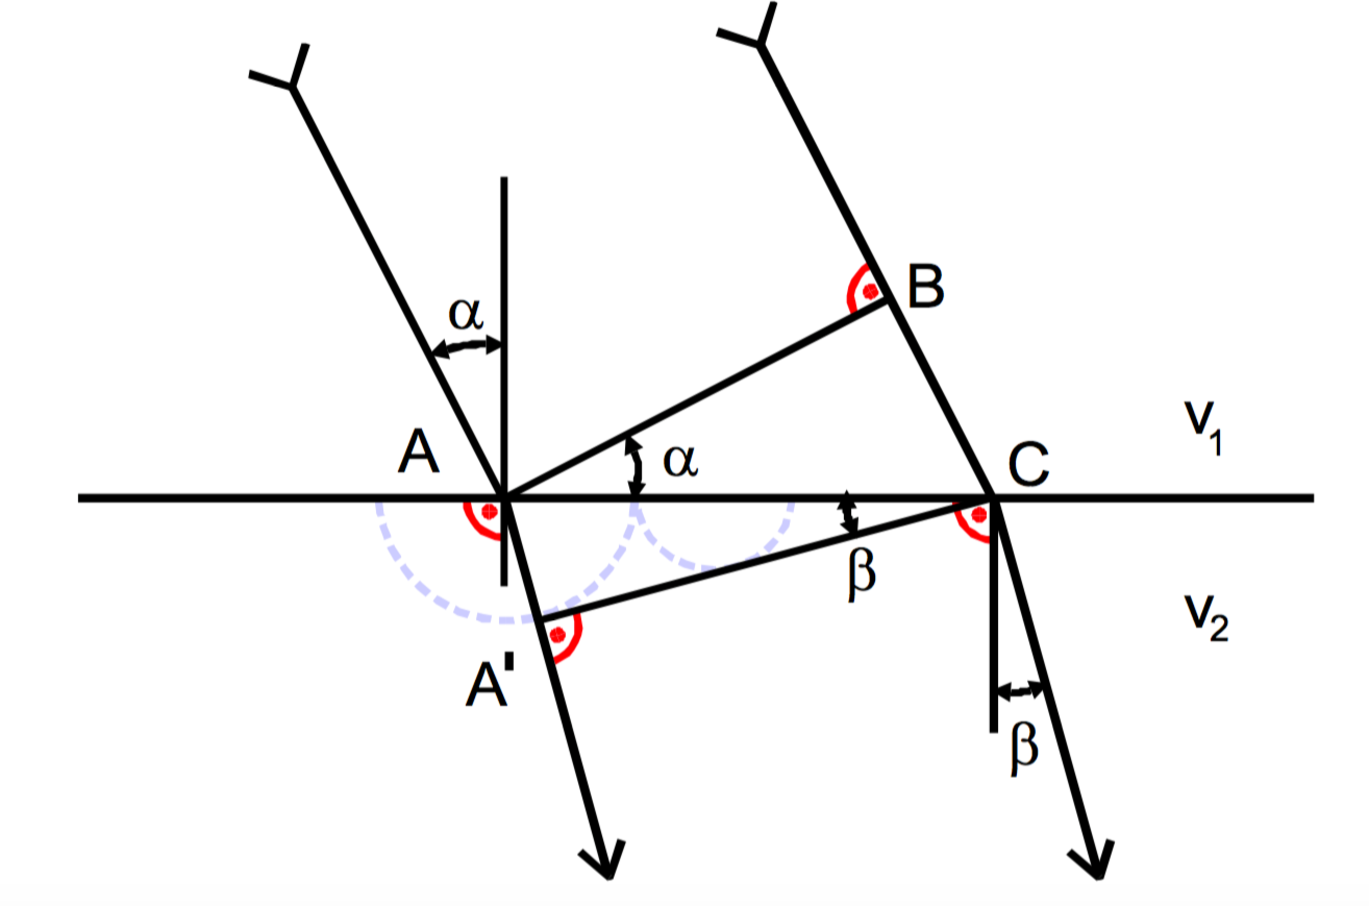
\includegraphics[width = 0.7\textwidth]{Pics/Snelius.pdf}
  \caption{Zur Ableitung des Snelliusschen Brechungsgesetzes mit Hilfe des Huygensschen Prinzips.}
  \label{fig:huygens}
\end{figure}

Der Brechungsindex lässt sich auch durch die Winkel beschreiben unter denen der Lichtstrahl
gebrochen wird. Dies kann mit dem Huygensschen Prinzip beschrieben werden. Es besagt, dass
jeder Punkt einer Wellenfläche als Ausgangspunkt einer elementaren Kugelwelle angesehen werden kann.
Wie in Abbildung \ref{fig:huygens} zu sehen, trifft die Wellenfront $AB$ schräg auf die Trennfläche.
Dadurch breiten sich im neuen Medium zu unterschiedlichen Zeitpunkten neue Kugelwellen aus, die sich
mit der Geschwindigkeit $v_2$ ausbreiten. Durch Überlagerung bilden sie nun
die Wellenfront $A^{'} C$. Aus der Abbildung lassen sich nun folgende Beziehungen ablesen:
\begin{equation*}
  \sin(\alpha) = \frac{\overline{B C}}{\overline{A C}} = \frac{v_1 T}{\overline{AC}} \text{~und~}
  \sin(\beta) = \frac{\overline{A^{'}A}}{\overline{A C}} = \frac{v_2 T}{\overline{A C}}.
\end{equation*}
Daraus folgt:
\begin{equation}
  \frac{\sin(\alpha)}{\sin(\beta)} = \frac{v_1}{v_2} = n.
  \label{eqn:snellius}
\end{equation}
Gleichung \eqref{eqn:snellius} heißt Snelliussches Brechungsgesetz.

\subsection{Ableitung der Dispersionsgleichung}

Nun wird die Dispersionsgleichung hergeleitet. Wie bereits erwähnt hängt diese Gleichung
von der Wellenlänge ab. Die Elektronen in dem Medium, in das die Lichtwelle eintritt,
werden in Schwingung versetzt. Dadurch kann die Absorbation des Lichtstrahls so
groß werden, dass die Dispersion nicht gut aufgenommen werden kann. Dieses Verhalten tritt
auf wenn die Wellenlänge des Lichts in der Nähe einer Resonanzstelle ist.
Glas, das in diesem Versuch verwendet wird, hat im infraroten und im ultravioletten Bereich des
Wellenlängenspektrums von Licht Resonanzstellen. Deshalb wird der Versuch mit Licht im sichtbaren
Bereich durchgeführt.
Die Schwingung der Elektronen kann durch folgende Differentialgleichung beschrieben werden:
\begin{equation}
  \underbrace{\frac{\g{d}^2 \vec{P}_\g{h}}{\g{d t}^2}}_{m_h \cdot a}
   + \underbrace{\frac{f_\g{h}}{m_\g{h}} \frac{\g{d}\vec{P}_\g{h}}{\g{d t}}}_{\text{Reibungskraft}}
   + \underbrace{\frac{a_\g{h}}{m_\g{h}}\vec{P}_\g{h}}_{\text{rücktreibende Kraft}}
   = \underbrace{\frac{N_\g{q} q_\g{h}^2}{m_\g{h}} \vec{E}_0 e^{i \omega t}}_{\text{periodische Kraft der elektromagnetischen Lichtwelle}}
   \label{eqn:DGL}
\end{equation}
Hierbei muss beachtet werden, dass die Erklärungen an einzelnen Termen nur aussagen sollen aus welcher Überlegung
dieser Term hergeleitet wurde. $\vec{P}_\g{h}$ ist die Polarisation eines Teilchens.
Nun können daraus die Dispersionsgleichungen hergeleitet werden. Sie beschreiben
den Real- und Imaginärteil der komplexen Größe $\tilde{n}^2$.
\begin{equation}
  \textbf{Re}(\tilde{n}^2) = n^2(1- k^2)
  = 1 + \sum_\g{h} \frac{N_\g{h} q_\g{h}^2 (\omega_\g{h}^2-\omega^2)}{\varepsilon~m_\g{h} \left( (\omega_\g{h}^2 - \omega^2)^2 + \frac{f_\g{h}^2}{m_\g{h}^2}\omega^2 \right)}
\end{equation}
und
\begin{equation}
   \textbf{Im}(\tilde{n}^2) = -2 n^2 k
   = \sum_\g{h} \frac{N_\g{h} q_\g{h}^2 f_\g{h}}{\varepsilon_0 m_\g{h}^2} \frac{\omega}{(\omega_\g{h}^2-\omega^2)^2 + \frac{f_\g{h}^2}{m_\g{h}^2} \omega^2 }.
\end{equation}
Nun wird die Dispersion weit weg von den Absorptionsstellen betrachtet. Es wird
außerdem angenommen, dass die Materie nur eine Absorptionsstelle $\lambda_1$ besitzt und
es gelte für Formel \eqref{eqn:zwischenformelfuertimo}: $\lambda >> \lambda_1$.
Dann kann $n^2(\lambda)$ mit einer Reihe nach Potenzen von $\frac{\lambda_1}{\lambda}$
geschrieben werden als:
\begin{equation}
  n^2(\lambda) = 1 + \frac{N_1 q_1^2 \lambda_1^2}{4 \pi^2 c^2 \varepsilon_0 m_1}
  \left( 1 + \left(\frac{\lambda_1}{\lambda}\right)^2 + \left(\frac{\lambda_1}{\lambda}\right)^4 + ...\right).
  \label{eqn:zwischenformelfuertimo}
\end{equation}

Kurz geschrieben liest sich dann:
\begin{equation}
  n^2(\lambda) = \g{A}_0 + \frac{\g{A_2}}{\lambda^2} + \frac{\g{A_4}}{\lambda^4} + ...
  \text{~mit~} \g{A}_0, \g{A}_2, \g{A}_4 > 0.
  \label{eqn:gestalta}
\end{equation}
Bei $\lambda << \lambda_1$ hat die Gleichung folgende Gestalt:
\begin{equation}
  n^2(\lambda) = 1- \g{A}_2^{'} \lambda^2 - \g{A}_4^{'} \lambda^4 - ...
  \text{~mit~} \g{A}_\g{i}^{'} > 0 \text{~für~} \g{i} \geq 2
  \label{eqn:gestaltb}
\end{equation}

Um zu entscheiden welche Gleichung die Dispersion besser beschreibt, wird
die Krümmung der zugehörigen Graphen aus Abbildung \ref{fig:Dispersionskurven}
betrachtet.
\begin{figure}
  \centering
  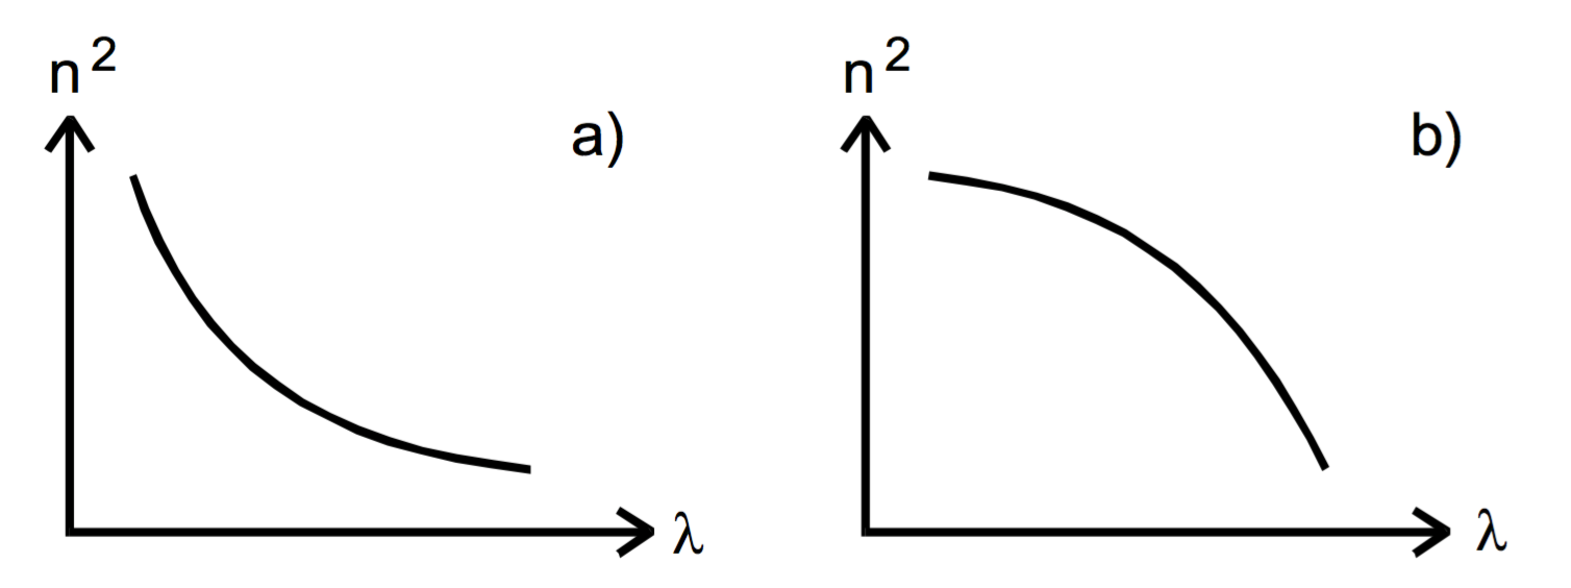
\includegraphics[width = \textwidth]{Pics/Dispersionskurven.pdf}
  \caption{Gestalt der Dispersionskurven a) nach \eqref{eqn:gestalta}, b) nach \eqref{eqn:gestaltb}.}
  \label{fig:Dispersionskurven}
\end{figure}
Dabei ist für \eqref{eqn:gestalta}:
\begin{align*}
  \frac{\g{d}^2 n^2(\lambda)}{\g{d} \lambda^2} &> 0\\
  \intertext{und für \eqref{eqn:gestaltb}}
  \frac{\g{d}^2 n^2(\lambda)}{\g{d} \lambda^2} &< 0
\end{align*}

Mit Hilfe der Dispersionsgleichung kann die Abbesche Zahl bestimmt werden.
Berechnet wird sie mit \eqref{eqn:abbe}.
\begin{equation}
  v = \frac{n_\g{D} -1 }{n_\g{F} - n_\g{C}}
  \label{eqn:abbe}
\end{equation}
$n_\g{D}, n_\g{F} \text{~und~} n_\g{C}$ sind hierbei die Brechungsindices zu den
Wellenlängen der Fraunhoferschen Linien: $\lambda_\g{C} = \SI{656}{\nano\meter},
\lambda_\g{D} = \SI{589}{\nano\meter} \text{~und~} \lambda_\g{F} = \SI{486}{\nano\meter}$.


\subsection{Auflösungsvermögen eines Prismen-Spektralapperats}

Das Auflösungsvermögen gibt an, wie groß der Wellenlängenunterschied $\Delta\lambda$ sein darf, damit
zwei Spektrallinien gerade noch getrennt werden können. Der Ausdruck ist dann:
\begin{equation*}
  A = \frac{\lambda}{\Delta\lambda}.
\end{equation*}

In diesem Versuch kann das Auflösungsvermögen mit folgender Formel bestimmt werden:
\begin{equation}
  \frac{\lambda}{\Delta\lambda} = b \frac{\g{d}n}{\g{d}\lambda}.
  \label{eqn:Aufloesung}
\end{equation}
Dabei ist $b$ die Basisbreite des Prismas.


\cite{anleitung}
